\section{Results}
\label{sec:results}

\subsection{Capability Floor Across Seven Arenas}

Table~\ref{tab:benchmark-results} is the primary empirical summary and reports all
seven benchmarks in one comparison; Table~\ref{tab:benchmark-definitions} defines
the task and metric for each row.

\begin{table}[H]
\centering
\scriptsize
\renewcommand{\arraystretch}{1.14}
\begin{tabularx}{\linewidth}{@{}p{1.55cm}p{1.55cm}p{1.10cm}X p{1.75cm}X@{}}
\toprule
\rowcolor{papersand}
\textbf{Benchmark} & \textbf{Backbone} & \textbf{Backend} & \textbf{Protocol} & \textbf{\systemname result} & \textbf{Comparison} \\
\midrule
SWE-Bench Pro & GPT-5.5/xhigh & Copilot & 731 software-repair tasks & $\approx$78\% accuracy & Direct Copilot $\approx$59\%; 1.41$\times$ aggregate Tokens \\
SOL-ExecBench & GPT-5.5 & Codex & B200; 101 kernels & Global \#6; 2$\times$\#1; 7 top-3 & Two head-to-head wins over Recursive \\
nanochat B200 & GPT-5.5 & Codex & 5 min; 1$\times$B200 & 0.9636 BPB & Human best 0.9646 \\
nanochat H100 & GPT-5.5 & Codex & 5 min; 1$\times$H100 & 0.9855 BPB & Human best 0.9879 \\
nanoGPT speedrun & GPT-5.5 & Codex & 8$\times$H100; $N{=}10$ & 79.77 s & Same-device human 80.18 s \\
AARRI-Bench & GPT-5.5 & Codex & 82 research-intern tasks & 63/82 (76.8\%) & Paper best 68.3\% \\
Math-Reasoning Data & GPT-5.5 & Codex & AIME-style synthesis & 28.0 gap & Arbor 20.83; Claude 8.33; Codex 6.25 \\
\bottomrule
\end{tabularx}
\caption{Results across seven benchmark arenas. Values remain in task-native units
and are not cross-normalized. Backbone denotes the model driving the research
agent; Backend denotes the execution surface.}
\label{tab:benchmark-results}
\end{table}

The runtime is not bound to one backbone or one execution surface. A separate
SWE-Bench Pro run replaces GPT-5.5 on Copilot with GLM-5.2 at a 200K-token context
window, driven through Claude Code, and is currently at 70.94\% accuracy. That run
is still in progress and has no matched Direct baseline on this backend, so we do
not enter it in Table~\ref{tab:benchmark-results} or in any longitudinal analysis;
we note it because the runtime carried the same contract, routing, and Reviewer
policy onto a different model and a different agent surface without
re-instrumentation.

As a small upstream-adoption example, an \systemname-optimized TileLang
\code{RWKV6} kernel was reviewed by a Moonshot AI-affiliated FLA collaborator and
merged into \code{fla-org:main}
(\href{https://github.com/fla-org/flash-linear-attention/pull/1045}{pull request (PR) \#1045};
\href{https://github.com/fla-org/flash-linear-attention/commit/c70f11c5530142450525549cc96d13d9f5165f69}
{commit \code{c70f11c}}); Appendix~\ref{app:upstream-kernel} records the technical
details.

An eighth arena is in progress and is reported here as a partial result. The
MLE-Bench Lite campaign runs the official MLE-Bench Low split
~\citep{chan2024mlebench} under a reviewer-approved medal gate: a competition counts
as complete only when an independently reviewed submission earns a Kaggle medal, so
the reported outcomes are medals rather than raw leaderboard positions.
Table~\ref{tab:mle-medals} lists the competitions closed to date: nine medals,
evenly split into three gold, three silver, and three bronze. The gate is narrow
rather than nominal. On \code{denoising-dirty-documents} the campaign settled
0.00009 RMSE short of the silver band, and on
\code{jigsaw-toxic-comment-classification-challenge} it cleared the bronze
threshold by 0.00018 AUC; both outcomes were awarded by the external grader
against the official Kaggle leaderboard, not by internal review. Two further
competitions were graded without reaching a medal: \code{dog-breed-identification}
finished above the median after twelve submissions, and
\code{new-york-city-taxi-fare-prediction} remained below it after four. The
transparent-conductor result is also a verification-gated route change: the
external grader rejected the initial approach at 0.208 RMSLE, the campaign
replaced it with a public-state-of-the-art method, and the grader then certified
the replacement inside the medal band at 0.06402 against a 0.06582 bronze
threshold. The remaining competitions continue to run; we exclude this arena from
Table~\ref{tab:benchmark-results} and will report the full split on completion.

\begin{table}[H]
\centering
\small
\renewcommand{\arraystretch}{1.18}
\begin{tabularx}{\linewidth}{@{}Xp{1.85cm}p{1.75cm}p{1.35cm}@{}}
\toprule
\rowcolor{papersand}
\textbf{Competition} & \textbf{Metric} & \textbf{\systemname} & \textbf{Medal} \\
\midrule
\code{aerial-cactus-identification} & AUC $\uparrow$ & \textbf{1.00000} & \textbf{Gold} \\
\code{dogs-vs-cats-redux-kernels-edition} & LogLoss $\downarrow$ & \textbf{0.02168} & \textbf{Gold} \\
\code{detecting-insults-in-social-commentary} & AUC $\uparrow$ & \textbf{0.91386} & \textbf{Gold} \\
\code{histopathologic-cancer-detection} & AUC $\uparrow$ & 0.98312 & Silver \\
\code{leaf-classification} & LogLoss $\downarrow$ & 0.00196 & Silver \\
\code{mlsp-2013-birds} & AUC $\uparrow$ & 0.91479 & Silver \\
\code{denoising-dirty-documents} & RMSE $\downarrow$ & 0.02618 & Bronze \\
\code{jigsaw-toxic-comment-classification-challenge} & AUC $\uparrow$ & 0.98657 & Bronze \\
\code{nomad2018-predict-transparent-conductors} & RMSLE $\downarrow$ & 0.06402 & Bronze \\
\bottomrule
\end{tabularx}
\caption{MLE-Bench Lite competitions closed with a medal by \systemname{} so far.
Arrows give the direction of improvement: area under the ROC curve (AUC) is
maximized, while log loss (LogLoss), root mean squared error (RMSE), and
column-wise root mean squared logarithmic error (RMSLE) are minimized. Each score
is the Reviewer-approved submission that the external MLE-Bench grader scored, and
each medal is the grader's award against that competition's official Kaggle
leaderboard. Seven of the nine rows are reconciled against the 2026-07-29
reviewer-approved campaign snapshot, which records 40 graded submissions across
nine competitions. The campaign is still running, so this table reports the
competitions closed to date rather than a final standing.}
\label{tab:mle-medals}
\end{table}

The table shows one runtime reaching competitive outcomes across heterogeneous
tasks. The remainder of this section
analyzes the SWE-Bench Pro row because it provides a long sequential trajectory and
Reviewer decisions.

\subsection{Knowing When to Stop: Verification Routing and Non-Termination}

Objective revision is admissible only if the runtime can withhold completion. This
subsection measures where independent verification is spent and where the runtime
declines to declare a task finished.

Of \ReviewerTasks{} tasks, \ReviewerInvoked{} (\ReviewerInvokedPercent\%) invoke
an independent Reviewer, while \ReviewerSkipped{} (\ReviewerSkippedPercent\%) use
Engineer self-review. The Reviewer requests another implementation round on
\ReviewerRevisionRequested{} tasks. After revision, \ReviewerVerifierRecovered{}
pass the official verifier and \ReviewerStrictRescues{} complete the strict
\code{continue}$\rightarrow$revision$\rightarrow$\code{done} loop. A further
\ReviewerFirstBlocked{} tasks receive a \code{blocked} verdict, recording that the
runtime cannot complete them rather than emitting an unsupported completion.
Refusing to stop early and refusing to claim success are two expressions of the same
gate.

Reviewer-routed tasks consume \ReviewerTokenRatio$\times$ as many solve input
tokens and \ReviewerTimeRatio$\times$ as much active time as self-reviewed tasks on
average, indicating that the routing policy selects a harder workload. The recovery
funnel is therefore more interpretable than a raw group-accuracy comparison.

Figure~\ref{fig:reviewer-mechanism} separates the routing population from the
revision-recovery path. The accepted and revise branches partition outcomes after
Reviewer invocation together with 35 blocked cases; verifier pass and strict rescue
are nested recovery milestones among the 43 revision-requested tasks.

\begin{figure}[H]
  \centering
  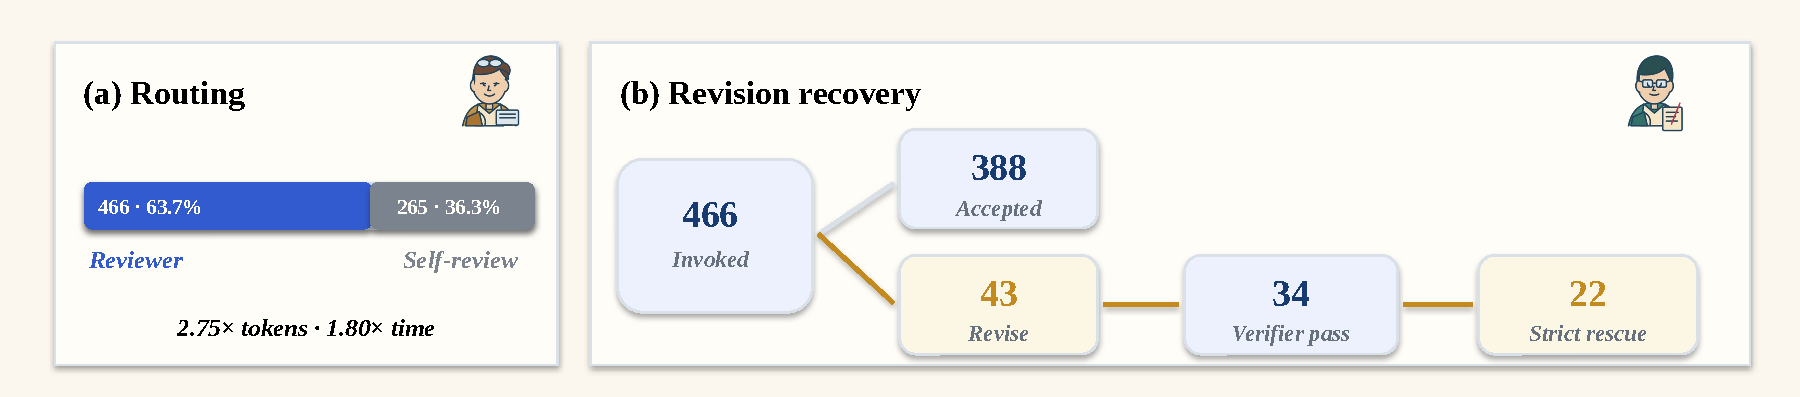
\includegraphics[width=\linewidth]{figures/reviewer_mechanism.pdf}
  \caption{Adaptive Reviewer routing and revision recovery. Panel (a) shows that
  466 of 731 tasks invoke an independent Reviewer, while 265 use Engineer
  self-review; routed tasks consume 2.75$\times$ the solve input Tokens and
  1.80$\times$ the active time on average. Panel (b) follows the routed workload:
  388 tasks are accepted on first review, 43 receive a revision request, 34 of
  those later pass the official verifier, and 22 complete the strict
  review-loop rescue. Routing is task-dependent; a randomized-routing run would
  additionally isolate the causal effect.}
  \label{fig:reviewer-mechanism}
\end{figure}

\subsection{Cost of the Mechanism as State Accumulates}

Figure~\ref{fig:swebench-evolution} shows the \systemname-only longitudinal
trajectory. Here, self-evolution refers to changes in persistent runtime state, not
to online training of the underlying model. Across Waves, accepted trajectories can
update repository knowledge, reusable Skills, verification guidance, task
definitions, and routing policy. These objects alter what later missions retrieve,
which checks they run, and where they spend independent review.

Mature operation W19--22 uses \SWEProTokenReduction\% fewer solve input Tokens and
\SWEProTimeReduction\% less active workflow time per task than startup W1--6. This
pattern is consistent with accumulated state reducing repeated inspection,
rediscovery, or failed execution. The lowest-Token window, W13--18, reaches a
\SWEProBestTokenReduction\% reduction from startup but requires more active time,
showing that Token efficiency and execution latency do not move together. The
final difficult-task window rebounds in both metrics.

\begin{figure}[H]
  \centering
  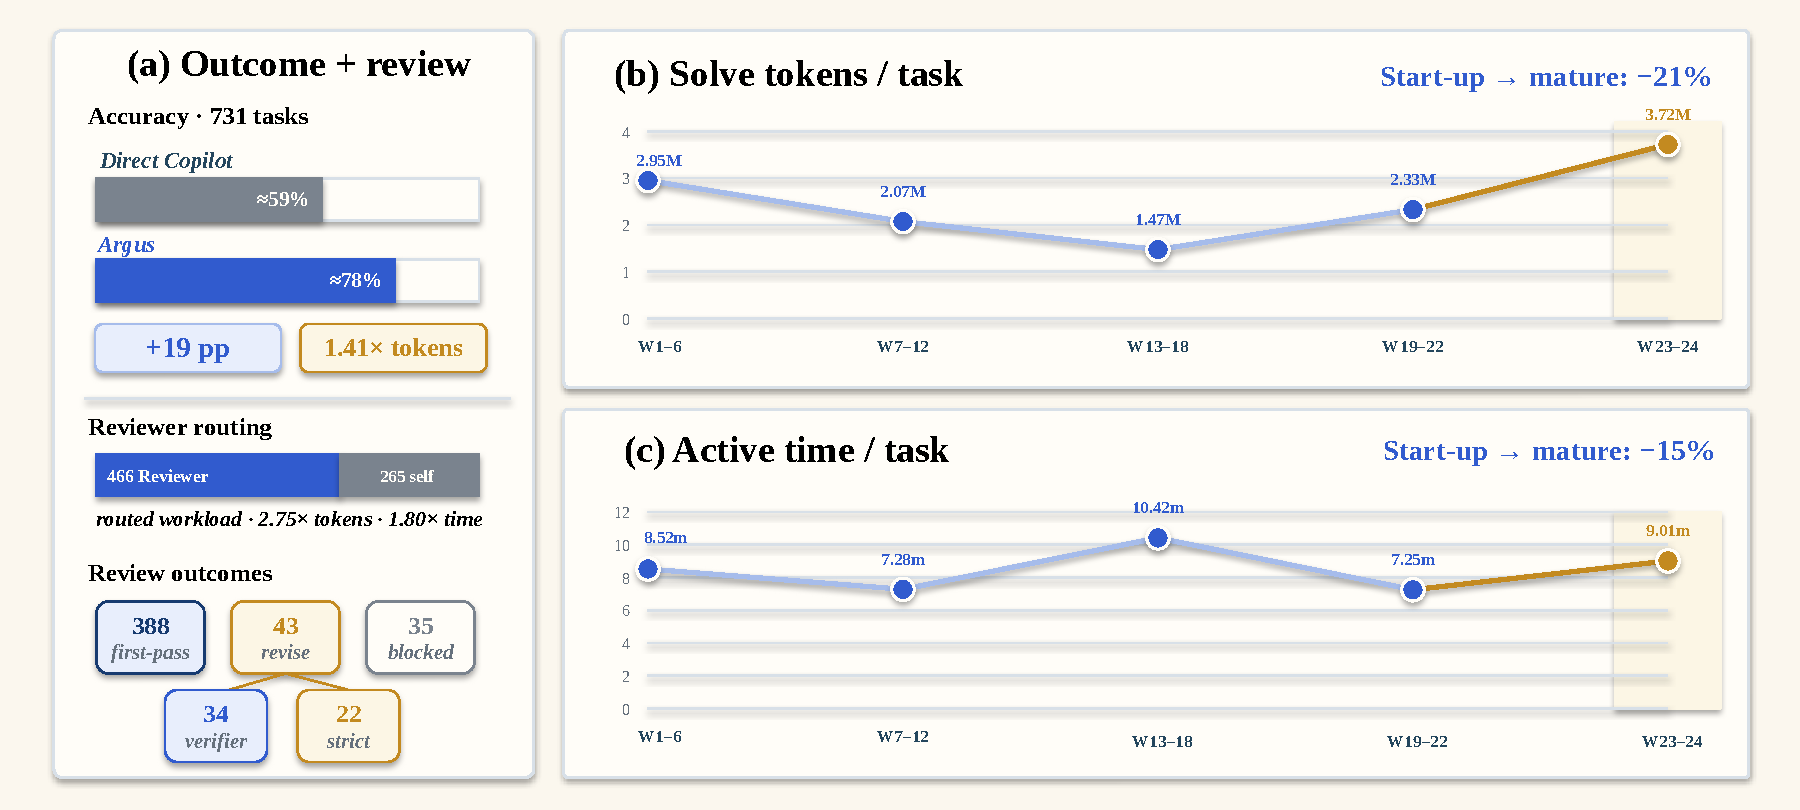
\includegraphics[width=\linewidth]{figures/swebench_evolution.pdf}
  \caption{Outcome, review, and longitudinal efficiency in the 731-task SWE-Bench
  Pro run. Panel (a) reports the full-suite accuracy and aggregate-Token comparison,
  adaptive Reviewer routing, and observed review outcomes. Panels (b) and (c)
  aggregate \systemname solve input Tokens and active workflow time over
  approximately six-Wave windows using task-weighted means. Relative to W1--6,
  W19--22 uses 21\% fewer solve input Tokens and 15\% less active time per task.
  Two incomplete Waves are omitted, while W23--24 remains visible as late
  difficult-task stress. Copilot per-Wave resource traces were not retained; the
  window comparison characterizes the operating profile over this sequence, and a
  controlled replay would isolate the learning effect.}
  \label{fig:swebench-evolution}
\end{figure}

The trajectories show a lower-cost mature operating window together with visible
task-composition and late-wave difficulty effects. The rebound in W23--24 prevents
the startup-to-mature comparison from being read as monotonic improvement. Because
the task sequence is not replayed against a frozen runtime state, the evidence
characterizes system-state accumulation over this sequence; attributing the
reduction to an individual memory or Skill update calls for a matched frozen-state
replay.

\subsection{Measured Process Quantities}

The process theory is instantiated from two complementary traces. In the
mathematical campaign, direct reasoning, verification, and action each account for
approximately 56\% of their respective attributed units. In SWE-Bench Pro, Reviewer
revision requests lead to 79.1\% official-verifier recovery and 51.2\% strict
review-loop rescue, while the mature window uses 21\% fewer solve input Tokens and
15\% less active time than startup. Appendix~\ref{app:formula-instantiation} gives
the complete substitutions for the density, reuse, yield, and compression
quantities.

The public research inventory additionally contains 41 de-duplicated artifacts
across six programs, illustrating the range of research programs executed by the
same runtime.
